\chapter{Periodograms}
\label{ch:axions-periodograms}
The space of possible axion--induced signals is spanned by their amplitude (the strength of the coupling) and their frequency (the axion mass). The problem is therefore naturally set in the frequency domain. We perform the analysis in two steps. First, we transform the measurements from the time domain into the frequency one by evaluating a \emph{periodogram} of it. The second step, the statistical treatment, is then easy.

In this section, we present the statistical methods we use. We start by defining the \emph{periodogram}, which serves as a transition from time to the frequency space, natural for looking for oscillations. Next we proceed to discuss the statistical properties of the periodogram, which lays the basis for this analysis.

For the sake of pedagogy we will discuss the methodology on a simple example.



\section{Definition}
A \emph{periodogram} is an estimator of the power spectrum. It has been proposed as the preferred way to treat periodic signals as early as 1898~\cite{Schuster1898}. In its simplest form it is the squared magnitude of the discrete Fourier transform. Lomb and Scargle have independently described a method one can construct a statistically well--behaving periodogram for non-uniformly sampled data with unequal error--bars: the Least Squares Spectral Analysis (LSSA)~\cite{Scargle1982}. It is also known as the Lomb--Scargle periodogram.

Many packages readily offer procedures to evaluate Lomb--Scargle periodograms~\cite{scipy,astropy}. They could not, however, be used directly as the analysis deviated in details from the standard procedure. We had to take a low--level approach, instead.

\begin{figure}
  \centering 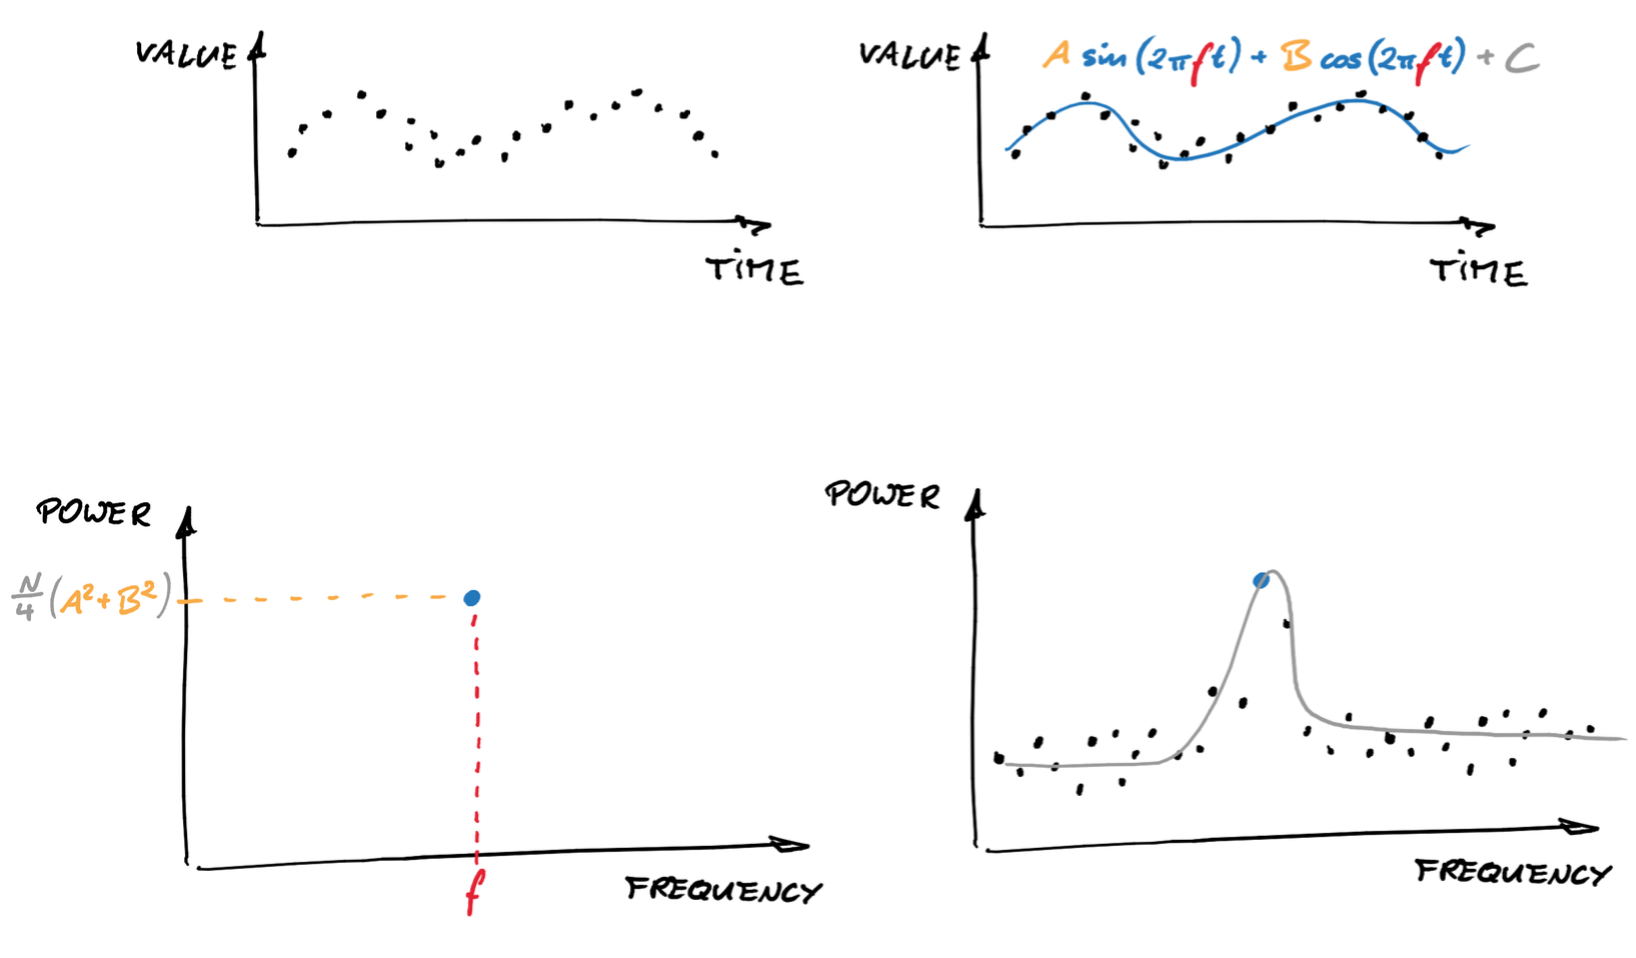
\includegraphics[width=\linewidth]{gfx/axions/LSSA}
  \caption{The LSSA periodogram, a function of frequency, is constructed by performing a linear least--squares fit at each of those frequencies.}
  \label{fig:LSSA_overview}
\end{figure}

To evaluate the LSSA periodogram at a circular frequency $\omega$, one performs a linear least--squares fit (hence the name) to the data with a function
\begin{equation}
  A\,\mathrm{cos}(\omega t) + B\,\mathrm{sin}(\omega t) + C \ ,
\end{equation}
where $A$, $B$ and $C$ are free parameters. The estimator of power $P(\omega)$ is then defined as
\begin{equation}
  P(\omega) := \frac{N}{4} \, \left( A^2 + B^2 \right) \ ,
\end{equation}
where $N$ is the number of data points. Different scaling factors may be used. We use the one of \cite{Scargle1982}, where the height of $\sqrt{P(\omega)}$ at the noise--bed corresponds numerically to the size of the error--bars squared, if they are all equal. LSSA, in contrast to the fast fourier transform (FFT), does not require windowing, because it is explicitly phase--aware. A graphical overview of the method is shown in Fig.\,\ref{fig:LSSA_overview}. Throughout the analysis, the figure of merit is either the power $P(\omega)$ or, interchangeably, its square root \emph{amplitude}. The latter has conveniently the same unit an the time series.

We will now follow an analysis of a simple example, shown in Fig.\,\ref{fig:basic_signal}. Despite being simple, is has already some properties of the actual dataset. The measurements are not equally spaced. They are grouped in 10--second long bunches, 20 seconds apart. Inside a bunch a measurement is taken every 2~seconds with a \unit[0.3]{s} jitter. The length of each measurement is 1~second with a \unit[0.1]{s} jitter. The error--bars are all size 1 in the arbitrary unit. An oscillating signal with an amplitude 0.7 and frequency \unit[0.17]{Hz}. Each measurement averages the signal over its duration.

\begin{figure}
  \centering 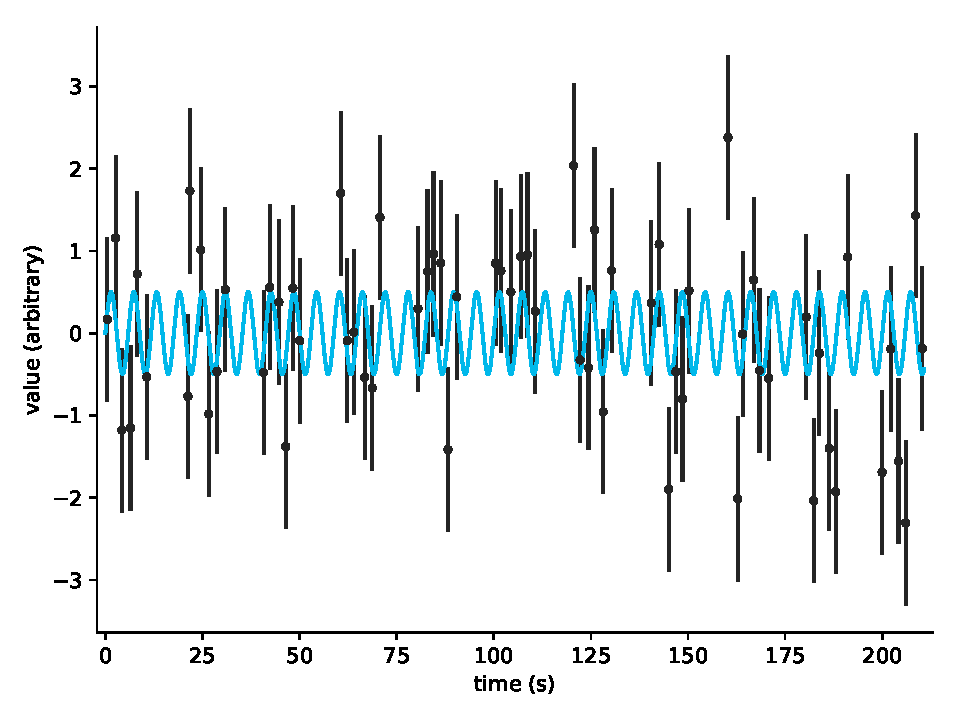
\includegraphics[width=0.8\linewidth]{gfx/axions/basic_signal.pdf}
  \caption{A simple signal generated just for the purpose for explaining the general scheme of the analysis.}
  \label{fig:basic_signal}
\end{figure}

We proceed to evaluate the LSSA periodogram of this time series. The immediate question is: for which frequencies to evaluate the power? In case of equally--spaced series the upper limit is the \emph{Nyquist frequency}, equal to the half of the sampling rate~\cite{Shannon1949}.

The \emph{spectral resolution} is the inverse span of the dataset and roughly defines the minimal frequency difference between two signals that is distinguishable. In Fig.\,\ref{fig:basic_periodogram} there are two periodograms: evaluated at frequencies spaced every spectral resolution (black dots), and one evaluated a thousand times more densely (orange line). We see that the structures are represented and the peak of the signal present in the data has finite width.

\begin{figure}
  \centering 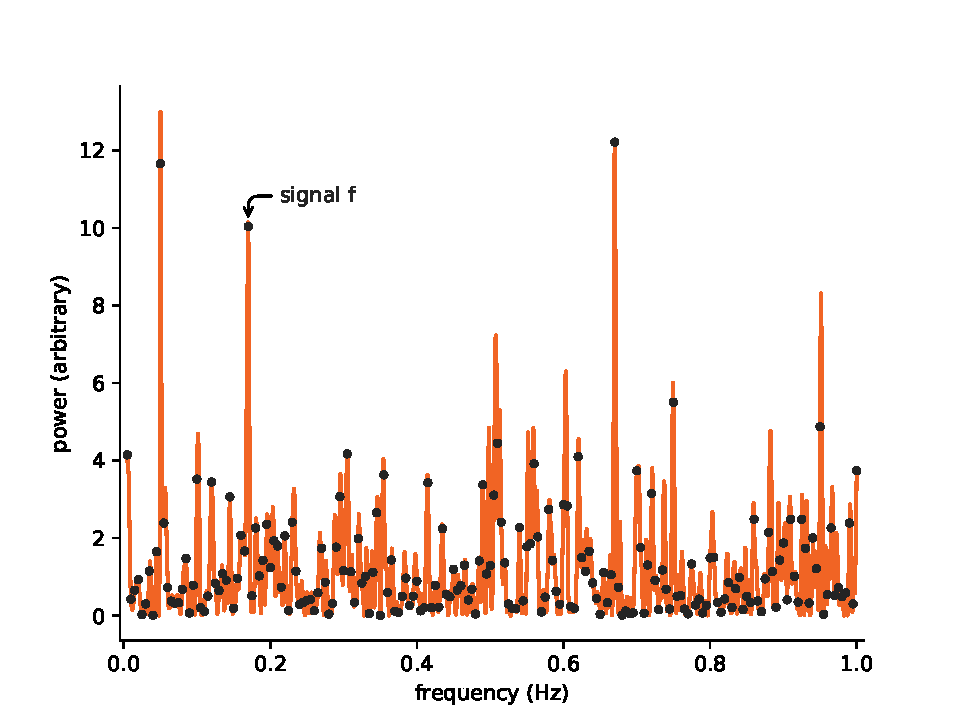
\includegraphics[width=0.8\linewidth]{gfx/axions/basic_periodogram.pdf}
  \caption{A simple signal generated just for the purpose for explaining the general scheme of the analysis.}
  \label{fig:basic_periodogram}
\end{figure}

Fig.\,\ref{fig:basic_periodogram_loglog} shows the same in a log--log scale. Often used, as the potential signals span orders of magnitude in both frequency and amplitude. But it can lead to misunderstanding. Consider for example noise, which appears to increase in amplitude for higher frequencies. Purely cognitive effect -- simply the density of points increases.

\begin{figure}
  \centering 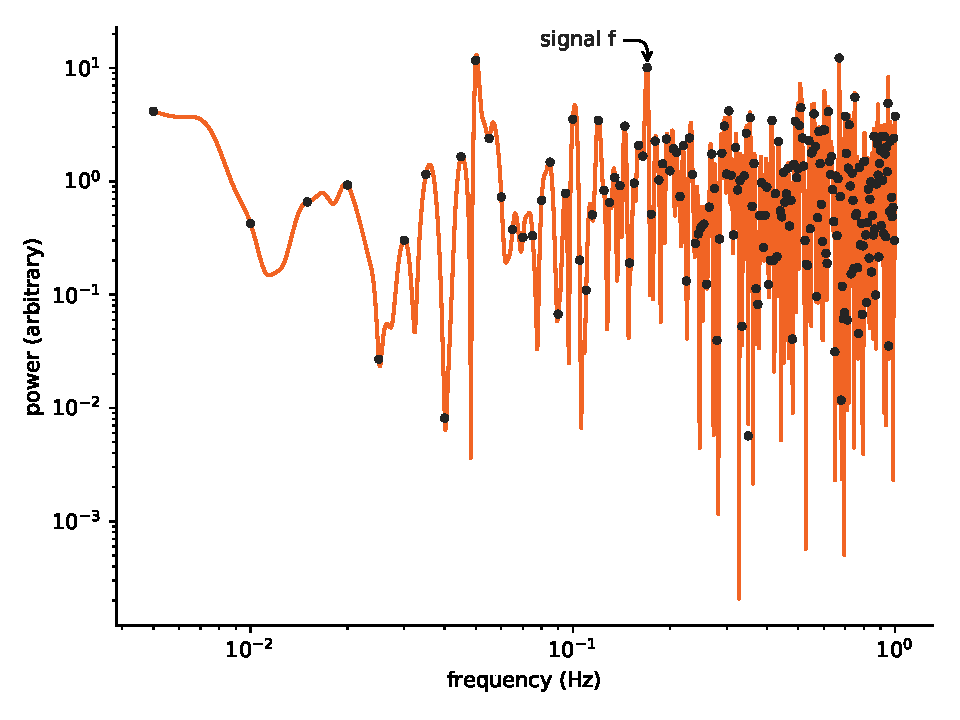
\includegraphics[width=0.8\linewidth]{gfx/axions/basic_periodogram_loglog.pdf}
  \caption{A simple signal generated just for the purpose for explaining the general scheme of the analysis.}
  \label{fig:basic_periodogram_loglog}
\end{figure}






\section{A null hypothesis test}
Once the periodogram of a time series is calculated we would like to know whether it contains a signal signature. A signature of a periodic signal is a peak in the periodogram. The really interesting statement is the answer to the question:

\begin{center}
  \emph{How likely it is, that the highest peak in the periodogram cannot be only~a~random~fluctuation?}
\end{center}

To describe the question mathematically, let us denote the time series from the real data by $D$. The peridogoram is then a set of $P^D(\omega_i)$. We are interested in \emph{the maximum of the periodogram}:
\begin{align}
  P_{max}^D &:= \mathrm{max}_i\,P^D(\omega_i) \\
  \omega_{max}^D &:= \mathrm{arg\,max}_i\,P^D(\omega_i)
\end{align}
The height of the maximum, $P_{max}^D$, is a random variable. We consider the distribution of $P_{max}$ given the null hypothesis, $H_0$, where an array of normally distributed random variables is taken. The probability that a peak at least as high as the one observed arises as a random fluctuation is:
\begin{equation}
  \mathrm{Pr}\left( P_{max} > P_{max}^D\ |\, H_0 \right) \ .
\end{equation}
This value is called the \emph{false alarm probability} (see eg. \cite{Pandola2004}). It can be numerically calculated with a Monte--Carlo method by generating random data according to the null hypothesis and counting the relative number of cases when $P_{max} > P_{max}^D$. To claim a discovery the \emph{false alarm probability} has to be at most in the range of $10^{-7}$ (so--called 5--sigma).

\begin{figure}
  \centering 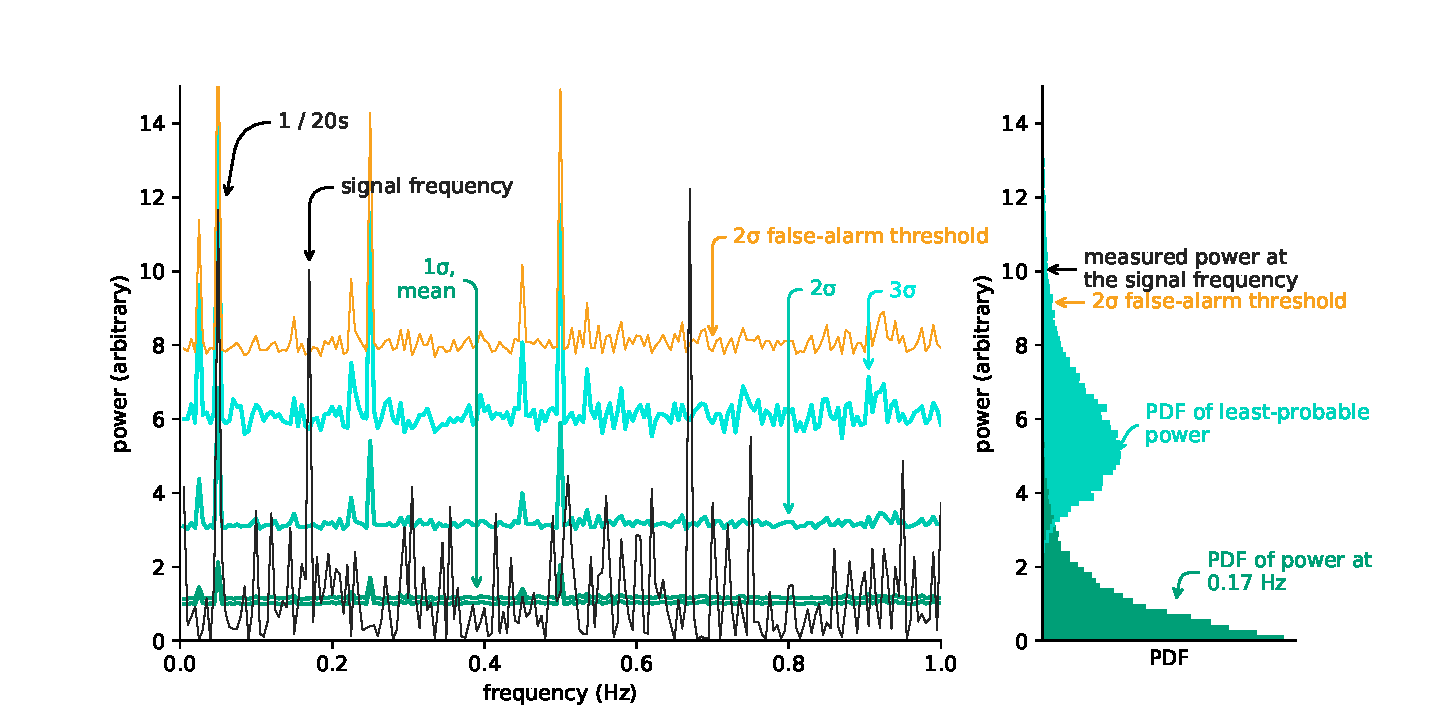
\includegraphics[width=\linewidth]{gfx/axions/basic_detection.pdf}
  \caption{A simple signal generated just for the purpose for explaining the general scheme of the analysis.}
  \label{fig:basic_detection}
\end{figure}

% \begin{figure}
%   \centering
%   \subfloat
%   % [The not--yet--real data tested against hypothetical signals. Each pixel is one signal hypothesis. The white line connects points of 95\% C.L., surrounding an exclusion region. Note how deep into low amplitudes the line goes for couple of frequencies. See the text for the explanation.]
%   {%\label{fig:axions_exclusion}
%   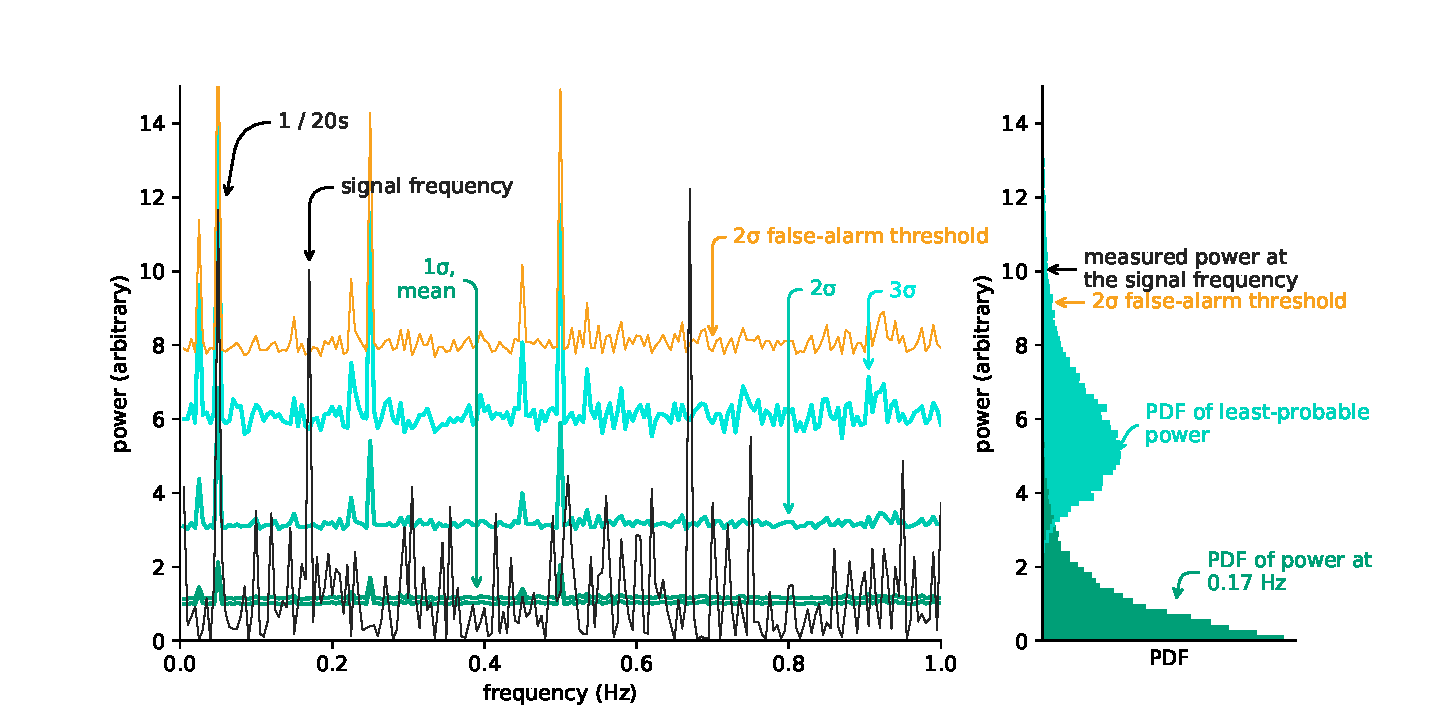
\includegraphics[width=.45\linewidth]{gfx/axions/basic_detection.pdf}}
%   \quad
%   \subfloat
%   % [The not--yet--real data tested against hypothetical signals using the \emph{CLs method}, in which hypotheses to which the experiment is not sensitive to get a statistical penalty. ]
%   {%\label{fig:basic_detection}
%   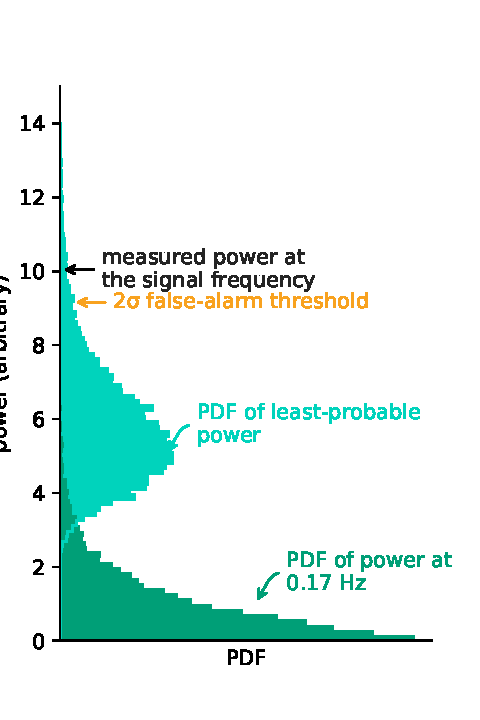
\includegraphics[width=.45\linewidth]{gfx/axions/basic_detection_histogram.pdf}}
%   \caption{Exclusion region --- signals that can be excluded at 95\% confidence level.}
%   \label{fig:basic_detection}
% \end{figure}

It should be emphasised that the distribution of $P_{max}$ is very different from the distribution of $P(\omega_{max})$. The highest peak will always occur in a far tail of the $P(\omega_{max})$ distribution, which is natural. By looking for the highest peak we check a big number of random variables $P(\omega_i)$ and pick the one that does lie the furthest in the tail of the distribution. The distribution of $P_{max}$ is centered around much higher values, as the highest peak is bound to occur \emph{somewhere}. It is explained in Fig.\,\ref{fig:axions_null_rejection}.


% \begin{figure}
%   \myfloatalign
%   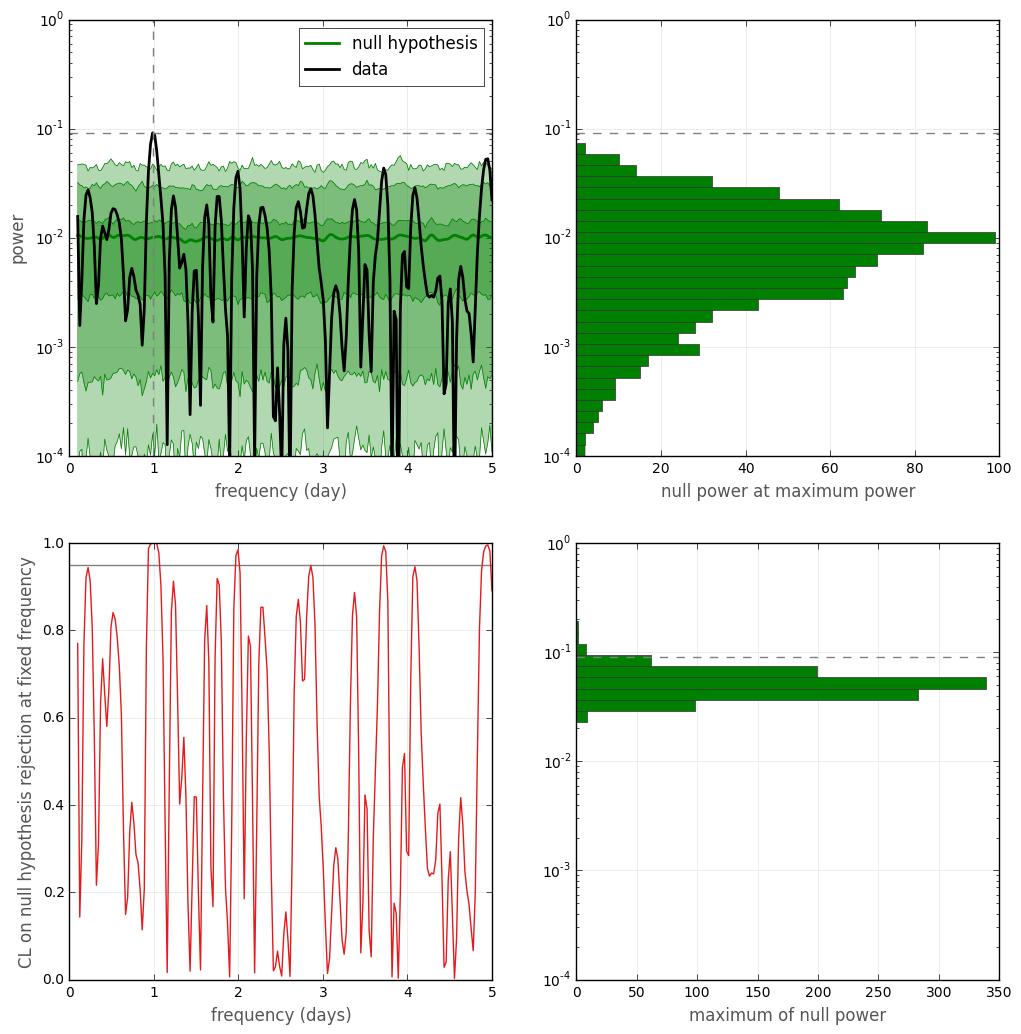
\includegraphics[width=.8\linewidth]{gfx/axions/axionMC_null_rejection}
%   \caption
%   [...]
%   {
% Testing not--yet--real data against the null hypothesis. \textsc{Upper--left:} The periodogram of the data (black line) on top of the periodogram of the null hypothesis (green line with Monte--Carlo generated distribution bands). \textsc{Upper--right:} The distribution of $P(\omega_{max})$, given the null hypothesis (vertical slice through the green part of the plot in the upper--left corner). \textsc{Lower--left:} CDF of $P(\omega)$ evaluated at $P^D(\omega)$ in function of $\omega$. \textsc{Lower--right:} The distribution of $P_{max}$. }
%   \label{fig:axions_null_rejection}
% \end{figure}





\section{Signal hypotheses tests}
Should no claim for a discovery be possible, the next question to ask is:
\begin{center}
  \emph{Which oscillations would produce a visible peak, but did not, and can be thus excluded?}
\end{center}
In order to answer this question, the data need to be tested against being compatible with a number of model signal hypotheses. As an oscillation is characterised by its amplitude and frequency, the space of the hypotheses to test is two--dimensional.

The probability that a hypothetical oscillation of amplitude $A$ and frequency $\omega$ would produce more power at $\omega$ then observed is:
\begin{equation}
  \mathrm{Pr}\left( P(\omega) > P^D(\omega)\ |\, H(\omega, A) \right) \ .
\end{equation}
This probability is the \emph{confidence level} (C.L.) at which the hypothesis $H(\omega, A)$ can be rejected. Figure\,\ref{fig:axions_signal_rejection} presents comparing a not--yet--real data power spectrum with a hypothetical signal. This test may be performed many times, each covering a \emph{pixel} of the space of possible hypotheses, forming an image as in Fig.\,\ref{fig:axions_exclusion}. The set of hypotheses excluded at a certain C.L. (often 95\%) forms an \emph{exclusion region}.

% \begin{figure}
%   \myfloatalign
%   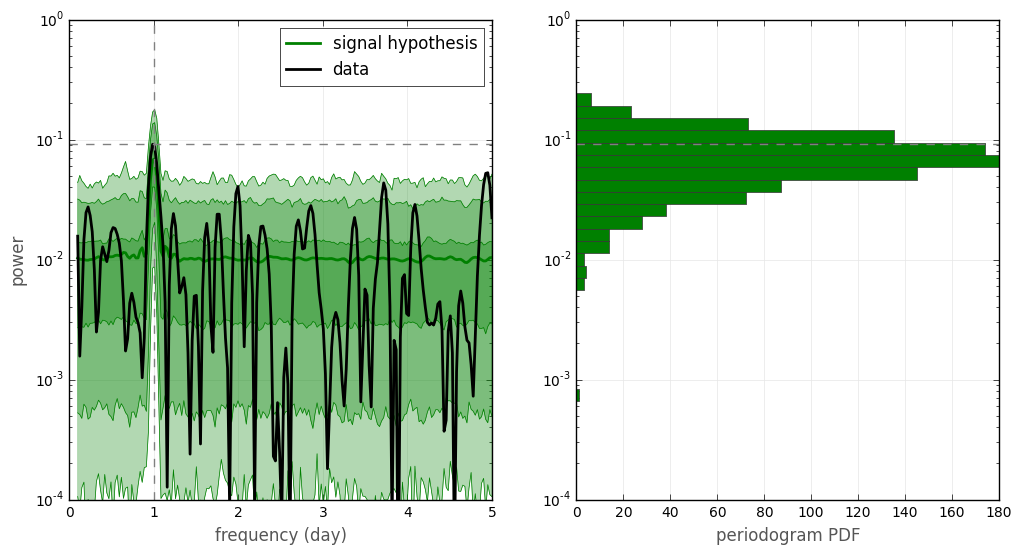
\includegraphics[width=.8\linewidth]{gfx/axions/axionMC_signal_hypothesis_rejection}
%   \caption
%   [...]
%   {
% \textsc{Left:} A periodogram of not--yet--real data on top of distribution of a periodogram of a hypothetical signal (green). \textsc{Right:} The distribution of power of the hypothetical signal at its model frequency.}
%   \label{fig:axions_signal_rejection}
% \end{figure}

\begin{figure}
  %FIXME directly copied from Elise's presentation on the 2015 PSI collaboration meeting
  \myfloatalign
  \subfloat
  [The not--yet--real data tested against hypothetical signals. Each pixel is one signal hypothesis. The white line connects points of 95\% C.L., surrounding an exclusion region. Note how deep into low amplitudes the line goes for couple of frequencies. See the text for the explanation.]
  {\label{fig:axions_exclusion_noCls}
  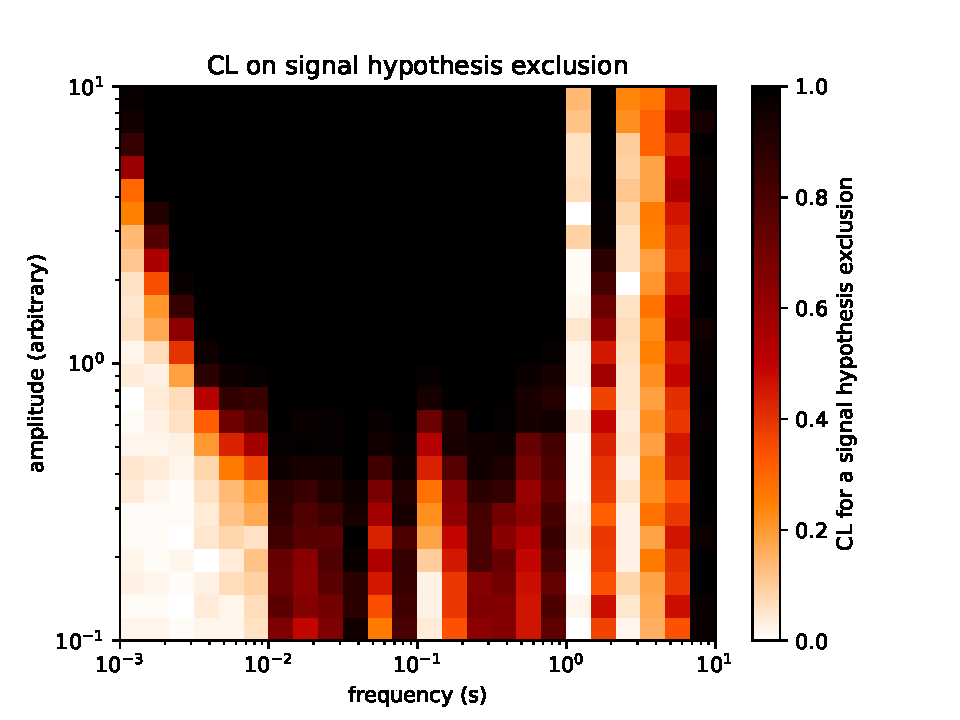
\includegraphics[width=.45\linewidth]{gfx/axions/basic_exclusion_noCls.pdf}}
  \quad
  \subfloat
  [The not--yet--real data tested against hypothetical signals using the \emph{CLs method}, in which hypotheses to which the experiment is not sensitive to get a statistical penalty. ]
  {\label{fig:axions_exclusion}
  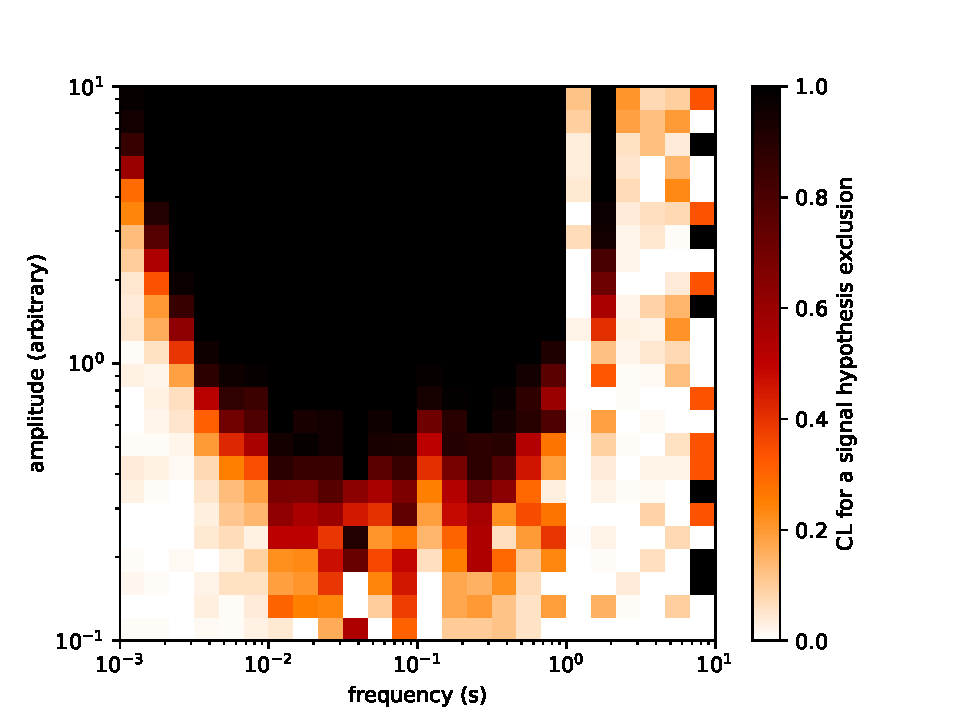
\includegraphics[width=.45\linewidth]{gfx/axions/basic_exclusion.pdf}}
  \caption{Exclusion region --- signals that can be excluded at 95\% confidence level..}
  \label{fig:axions_exclusions}
\end{figure}

The exclusion region, depicted by a white line in Fig.\,\ref{fig:axions_exclusion}, is exhibits a number of thin peaks going down in very low amplitudes. Seemingly for some frequencies signals with amplitude far below the sensitivity of the experiment are excluded. This is disturbing. Consider, however, that as the power was evaluated for many frequencies, inevitably at some of them, roughly 5\%, the power is low enough to be rejected at 95\%~C.L. even when tested against a white noise. However completely fine from the statistical point of view, physicists do not accept a situation, where a hypothesis is rejected based on an experiment which was not sensitive to it. One possible solution is called the \emph{CLs method}. The method is defined, as well the problem itself discussed, in the booklet of Particle Data Group~\citep{Group2014}. With use of the \emph{CLs method} the exclusion final region is obtained, as shown in Fig.\,\ref{fig:axions_exclusion_CLs}.
